% =====================================================================
%  V2V-Project -- Study Pack
%  Section S8 : Attack Demonstrations
%  Source files: attacks/replay_attack.py, tamper_attack.py, mitm_attack.py
%  Standalone document -- compile with:  pdflatex 08-attack-demonstrations.tex
% =====================================================================
\documentclass[11pt,a4paper]{article}

\usepackage[utf8]{inputenc}
\usepackage[T1]{fontenc}
\usepackage{lmodern}

\usepackage[a4paper,margin=2.4cm]{geometry}
\usepackage{enumitem}
\setlist{topsep=2pt,itemsep=2pt}

\usepackage{amsmath}
\usepackage{amssymb}
\usepackage{booktabs}
\usepackage{graphicx}
\usepackage{xcolor}
\usepackage{listings}
\usepackage{tikz}
\usetikzlibrary{arrows.meta,positioning,shapes.geometric,calc,fit,backgrounds}
\usepackage[colorlinks=true,linkcolor=blue,urlcolor=blue,citecolor=blue]{hyperref}

\definecolor{codebg}{rgb}{0.97,0.97,0.94}
\definecolor{codegreen}{rgb}{0.00,0.50,0.00}
\definecolor{codegray}{rgb}{0.50,0.50,0.50}
\definecolor{keyblue}{rgb}{0.00,0.20,0.70}
\definecolor{boxblue}{rgb}{0.88,0.93,1.00}
\definecolor{boxyellow}{rgb}{1.00,0.97,0.85}

\lstdefinestyle{py}{
  language=Python,
  backgroundcolor=\color{codebg},
  basicstyle=\ttfamily\footnotesize,
  keywordstyle=\color{keyblue}\bfseries,
  stringstyle=\color{codegreen},
  commentstyle=\color{codegray}\itshape,
  numberstyle=\tiny\color{codegray},
  numbers=left,
  numbersep=8pt,
  showstringspaces=false,
  breaklines=true,
  breakatwhitespace=false,
  frame=single,
  rulecolor=\color{codegray},
  tabsize=4,
  captionpos=b,
}
\lstdefinestyle{term}{
  backgroundcolor=\color{codebg},
  basicstyle=\ttfamily\footnotesize,
  breaklines=true,
  frame=single,
  rulecolor=\color{codegray},
  numbers=none,
  captionpos=b,
}

\title{\textbf{V2V-Project Study Pack}\\[4pt]
       \large Section S8 --- Attack Demonstrations}
\author{Information Security Project --- Beginner Study Notes}
\date{Source files: \texttt{attacks/replay\_attack.py}, \texttt{tamper\_attack.py}, \texttt{mitm\_attack.py}}

\begin{document}
\maketitle
\tableofcontents
\newpage

% =====================================================================
\section{Title and ``What You'll Learn''}
% =====================================================================

\subsection*{Section Title}
\textbf{S8 --- Attack Demonstrations: three short scripts that play the role of
the attacker and prove, on screen, that the defences actually work.}

\subsection*{Plain-English Summary (read this first)}
A security claim means nothing until you \emph{try to break it}. Section~S8 is
the project's ``red team'': three Python scripts that each \emph{become the
attacker}. \texttt{replay\_attack.py} captures a real message and re-sends it
late. \texttt{tamper\_attack.py} intercepts a message and flips bits in it.
\texttt{mitm\_attack.py} plays the man-in-the-middle in two ways --- a fake
certificate and a forged signature. Each script runs the attack against the real
project code and prints \texttt{[BLOCKED]} when the defence stops it. S8 does not
add any new defence --- it \emph{tests} the defences of S2--S5.

\subsection*{Learning Outcomes}
After studying this section you will be able to:
\begin{itemize}
  \item Explain \textbf{adversarial testing} (red-teaming) and why it matters.
  \item Describe exactly how a \textbf{replay}, a \textbf{tamper} and a
        \textbf{man-in-the-middle} attack are performed.
  \item Walk through each attack script step by step.
  \item Name the precise defence (and which section) that blocks each attack.
  \item Run all three scripts, read their output, and explain every line.
  \item Honestly explain the limits of each demonstration.
\end{itemize}

% =====================================================================
\section{Where This Fits}
% =====================================================================

S8 sits \emph{against} the whole pipeline. The earlier sections \emph{claim}
six security properties; S8 is where those claims are put on trial. Each script
imports the real project modules --- the same \texttt{crypto.py},
\texttt{auth\_protocol.py} and \texttt{v2v\_protocol.py} the vehicles use --- and
attacks them. If a defence were broken, the script would print \texttt{[FAIL]}.

\begin{center}
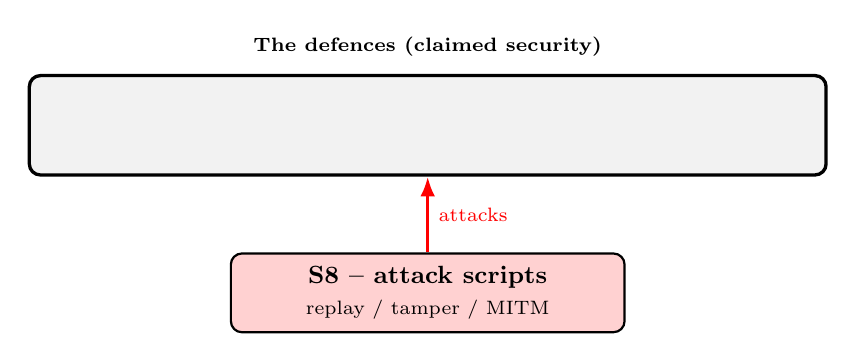
\begin{tikzpicture}[font=\small,node distance=7mm and 10mm,
   st/.style={draw,rounded corners,minimum width=2.6cm,minimum height=1.0cm,
              align=center,thick}]
  \node[st,fill=boxblue]   (id)   {Identity\\\scriptsize S2};
  \node[st,fill=green!12,right=of id]   (au) {Authentication\\\scriptsize S4};
  \node[st,fill=boxyellow,right=of au] (ms) {Messaging\\\scriptsize S5};
  \node[draw,very thick,rounded corners,fill=gray!10,fit=(id)(au)(ms)] (def) {};
  \node[above=1mm of def,font=\scriptsize\bfseries] {The defences (claimed security)};
  \node[st,fill=red!18,below=11mm of au,minimum width=5cm] (atk)
       {\textbf{S8 -- attack scripts}\\\scriptsize replay / tamper / MITM};
  \draw[-{Latex[length=2.5mm]},very thick,red] (atk) -- (def)
       node[midway,right,font=\scriptsize]{attacks};
\end{tikzpicture}
\end{center}

% =====================================================================
\section{The Theory You Must Study}
% =====================================================================

\subsection{Adversarial Testing (Red-Teaming)}
\textbf{Plain definition.} \emph{Adversarial testing} means deliberately
attacking your own system to check the defences hold. A \emph{red team} is the
group (or here, the scripts) that plays the attacker.

\textbf{Real-life analogy.} A locksmith does not just \emph{say} a lock is good
--- they hire someone to try every trick to pick it. If it opens, the lock is
not good.

\textbf{Why it exists.} Designers are optimistic; they trust their own code. An
attacker is not bound by the designer's assumptions. Testing from the attacker's
side finds the gap between ``should be secure'' and ``is secure''.

\textbf{How it works here.} Three scripts each import the genuine project modules
and perform a real attack against them, then report \texttt{[BLOCKED]} or
\texttt{[FAIL]}.

\textbf{Security property it relates to.} It validates \emph{all} of them ---
S8 is the evidence behind the project's security claims.

\subsection{The Replay Attack}
\textbf{Plain definition.} The attacker records a genuine, valid encrypted
message and sends the \emph{exact same bytes} again later.

\textbf{Real-life analogy.} Secretly recording someone saying ``open the garage''
and playing the recording back tomorrow.

\textbf{Why it is dangerous.} The replayed message is \emph{perfectly valid} ---
correct encryption, correct signature. Nothing is forged. The only thing wrong is
that it is \emph{old}. Re-sending an old ``I am braking!'' could trigger needless
braking and a crash.

\textbf{How the script does it.} \texttt{replay\_attack.py} sends a BSM, lets it
be received once (which succeeds), waits \textbf{6 seconds} --- one second past
the 5-second freshness window --- then re-sends the identical bytes.

\textbf{The defence that stops it.} The \texttt{TimestampValidator} (S4/S5): the
message's timestamp is now more than 5 seconds old, so
\texttt{secure\_receive} raises \texttt{StaleMessageError}. The sequence-number
check is a second line of defence.

\subsection{The Tamper Attack}
\textbf{Plain definition.} The attacker intercepts a message in transit and
changes some of its bytes.

\textbf{Real-life analogy.} Steaming open a sealed envelope, editing the letter,
and trying to re-seal it --- but the seal is mathematical and cannot be re-made.

\textbf{Why it is dangerous.} If tampering went undetected, an attacker could
turn ``speed 85'' into ``speed 0'' and mislead other cars.

\textbf{How the script does it.} \texttt{tamper\_attack.py} encrypts a BSM, then
flips \textbf{3 random bytes} in the packet (deliberately past the header, in the
ciphertext region), and tries to receive it.

\textbf{The defence that stops it.} AES-256-GCM's authentication tag (S3, used by
S5): the tag no longer matches the changed ciphertext, \texttt{aes\_gcm\_decrypt}
raises \texttt{DecryptionError}, and \texttt{secure\_receive} turns it into a
\texttt{TamperError}.

\subsection{The Man-in-the-Middle (MITM) Attack}
\textbf{Plain definition.} The attacker secretly positions themselves between the
two cars and tries to impersonate one of them.

\textbf{Real-life analogy.} A dishonest interpreter between two people who do not
share a language --- each trusts the interpreter completely.

\textbf{Why it is dangerous.} A successful MITM could read and rewrite the entire
conversation.

\textbf{How the script does it --- two scenarios.}
\begin{itemize}
  \item \textbf{Scenario A --- fake certificate.} The attacker makes their own
        \emph{self-signed} certificate that claims the name \texttt{vehicle-a}.
  \item \textbf{Scenario B --- forged signature.} The attacker lets the real
        certificates through but tries to answer the handshake challenge by
        signing the nonces with \emph{their own} private key.
\end{itemize}

\textbf{The defences that stop it.}
\begin{itemize}
  \item Scenario~A: \texttt{verify\_certificate\_against\_ca} (S2/S4) checks the
        CA's signature. A self-signed forgery was not signed by the CA, so it
        raises \texttt{CertificateError}.
  \item Scenario~B: \texttt{ecdsa\_verify} (S3/S4) checks the challenge signature
        with \texttt{vehicle-a}'s \emph{real} public key. A signature made with
        the attacker's key does not verify, so it returns \texttt{False}.
\end{itemize}

\subsection{Self-Signed Forgery vs CA-Signed Trust}
A genuine vehicle certificate is signed by the \textbf{CA}'s private key. The
attacker does not have that key, so the best they can do is a \emph{self-signed}
certificate --- one signed by their own key, where issuer and subject are the
same. It \emph{looks} like a certificate, but the chain of trust check
(``did the CA sign this?'') fails immediately. \emph{This is the heart of
Scenario~A.}

% =====================================================================
\section{Code Walkthrough}
% =====================================================================

\subsection{File: attacks/replay\_attack.py}
\textbf{One-line purpose:} capture a valid BSM, wait past the freshness window,
replay it, and show it is rejected.
\begin{lstlisting}[style=py,caption={replay\_attack.py --- the replay attack (key parts).}]
def main() -> None:
    # Setup: shared session key + signing keys
    priv_a, pub_a = generate_ecdh_keypair()
    priv_b, pub_b = generate_ecdh_keypair()
    secret = ecdh_shared_secret(priv_a, pub_b)
    session_key = derive_session_key(secret, os.urandom(16), os.urandom(16))
    sign_key = generate_private_key(SECP256R1())
    verify_key = sign_key.public_key()

    # Step 1: Vehicle A sends a legitimate BSM
    bsm = BasicSafetyMessage("vehicle-a", 80.0, 45.0, 6.9271, 79.8612,
                             time.time(), 1, False)
    raw_bytes = secure_send(bsm, session_key, sign_key, logger)

    # Step 2: First delivery -- should PASS
    received = secure_receive(raw_bytes, session_key, verify_key,
                              ReplayCache(), TimestampValidator(5.0), logger2)

    # Step 3: Wait 6 seconds (beyond the 5-second window)
    time.sleep(6)

    # Step 4: Replay the exact same bytes
    try:
        secure_receive(raw_bytes, session_key, verify_key,
                       ReplayCache(), TimestampValidator(5.0), logger3, last_seq=0)
        print("[FAIL] Replayed message was ACCEPTED")
    except (StaleMessageError, SequenceError) as e:
        print(f"[BLOCKED] Replay attempt REJECTED -- Reason: {e}")
\end{lstlisting}
\textbf{Step by step:}
\begin{enumerate}
  \item \textbf{Setup} --- it builds a session key with ECDH+HKDF (simulating a
        finished handshake) and an ECDSA signing key, so there is a working
        secure channel to attack.
  \item \textbf{Step 1} --- it creates a BSM and calls \texttt{secure\_send}; the
        comment in the script calls this the ``\texttt{[CAPTURED]}'' message ---
        the bytes an attacker would have recorded.
  \item \textbf{Step 2} --- it delivers the bytes once with
        \texttt{secure\_receive}. This \emph{succeeds}, proving the message is
        genuinely valid.
  \item \textbf{Step 3} --- \texttt{time.sleep(6)} waits 6 seconds, one second
        past the 5-second freshness window.
  \item \textbf{Step 4} --- it calls \texttt{secure\_receive} again with the
        \emph{same} bytes. The timestamp is now stale, so a
        \texttt{StaleMessageError} is raised, caught, and reported as
        \texttt{[BLOCKED]}.
\end{enumerate}
\textbf{Honest note on this demo.} Each call uses a \emph{fresh}
\texttt{ReplayCache}, and recall from S5 that \texttt{secure\_receive} does not
actually consult the nonce cache --- so in this isolated script the
\emph{timestamp} (and the sequence check) is what blocks the replay. The nonce
cache is real, but it is used in the \emph{handshake} (S4), not the BSM path. The
script's final report lists the nonce cache as a defence; that is true of the
system as a whole, but it is the timestamp that fires \emph{in this script}.
\textbf{Theory link:} replay attack vs the timestamp freshness window.

\subsection{File: attacks/tamper\_attack.py}
\textbf{One-line purpose:} encrypt a BSM, flip bits in the ciphertext, and show
the tampered message is rejected while the original still works.
\begin{lstlisting}[style=py,caption={tamper\_attack.py --- the tamper attack (key parts).}]
def main() -> None:
    # Setup: session key + signing keys (as in replay_attack)
    ...
    # Step 1: create and encrypt a legitimate BSM
    bsm = BasicSafetyMessage("vehicle-a", 85.3, 90.0, 6.9271, 79.8612,
                             time.time(), 1, True)
    raw_bytes = secure_send(bsm, session_key, sign_key, logger1)

    # Step 2: tamper -- flip 3 random bytes in the ciphertext region
    tampered = bytearray(raw_bytes)
    safe_start = 30                       # skip the header fields
    positions = [random.randint(safe_start, len(tampered) - 1) for _ in range(3)]
    for pos in positions:
        tampered[pos] ^= 0xFF

    # Step 3: attempt to decrypt the tampered message
    try:
        secure_receive(bytes(tampered), session_key, verify_key,
                       ReplayCache(), TimestampValidator(5.0), logger2)
        print("[FAIL] Tampered message was ACCEPTED")
    except TamperError as e:
        print(f"[BLOCKED] Tampered message REJECTED -- Reason: {e}")

    # Step 4: verify the ORIGINAL (untampered) message still works
    received = secure_receive(raw_bytes, session_key, verify_key,
                              ReplayCache(), TimestampValidator(5.0), logger3)
\end{lstlisting}
\textbf{Step by step:}
\begin{enumerate}
  \item \textbf{Setup + Step 1} --- build a session key and a signed, encrypted
        BSM, exactly as a sender would.
  \item \textbf{Step 2} --- copy the wire bytes into a mutable \texttt{bytearray},
        pick 3 random positions \emph{after byte 30} (so the flips land in the
        ciphertext, not the header), and flip each with \texttt{\^{}= 0xFF} (XOR
        with all-ones inverts every bit of that byte).
  \item \textbf{Step 3} --- feed the tampered bytes to \texttt{secure\_receive}.
        AES-GCM recomputes the authentication tag, finds a mismatch, and
        \texttt{secure\_receive} raises \texttt{TamperError} --- reported as
        \texttt{[BLOCKED]}.
  \item \textbf{Step 4} --- it decrypts the \emph{original} (untouched) bytes to
        prove the channel itself is fine; only the tampered copy fails. This is
        an important control: it shows the rejection is caused by the tampering,
        not by a broken setup.
\end{enumerate}
\textbf{Theory link:} AES-256-GCM authenticated encryption --- the 16-byte tag
makes the message tamper-evident.

\subsection{File: attacks/mitm\_attack.py}
\textbf{One-line purpose:} run a man-in-the-middle attack two ways --- a fake
certificate and a forged signature --- and show both are rejected.

\subsubsection*{\_make\_fake\_cert() --- forge a self-signed certificate}
\begin{lstlisting}[style=py,caption={mitm\_attack.py --- building a fake (self-signed) certificate.}]
def _make_fake_cert(common_name="vehicle-a"):
    fake_key = generate_private_key(SECP256R1())
    subject = x509.Name([
        x509.NameAttribute(NameOID.COMMON_NAME, common_name),
        x509.NameAttribute(NameOID.ORGANIZATION_NAME, "V2V-Security-Lab"),
    ])
    cert = (x509.CertificateBuilder()
        .subject_name(subject)
        .issuer_name(subject)               # self-signed -- NOT signed by the CA
        .public_key(fake_key.public_key())
        .serial_number(x509.random_serial_number())
        .not_valid_before(datetime.utcnow())
        .not_valid_after(datetime.utcnow() + timedelta(days=365))
        .add_extension(x509.BasicConstraints(ca=False, path_length=None), critical=True)
        .sign(private_key=fake_key, algorithm=hashes.SHA256()))
    return cert.public_bytes(serialization.Encoding.PEM), fake_key
\end{lstlisting}
\textbf{Step by step:} the attacker generates their own key, builds a certificate
that \emph{names} \texttt{vehicle-a}, and --- crucially --- sets
\texttt{issuer\_name} equal to \texttt{subject\_name} and signs it with their own
key. It is \emph{self-signed}. It looks like a certificate but carries the
attacker's signature, not the CA's.

\subsubsection*{main() --- the two scenarios}
\begin{lstlisting}[style=py,caption={mitm\_attack.py --- the two MITM scenarios (key parts).}]
# SCENARIO A: certificate replacement
fake_cert_pem, fake_key = _make_fake_cert("vehicle-a")
try:
    verify_certificate_against_ca(fake_cert_pem.decode(), ca_pem)
    print("[FAIL] Fake certificate was ACCEPTED")
except CertificateError as e:
    print(f"[BLOCKED] Fake certificate REJECTED -- Reason: {e}")

# SCENARIO B: signature forgery
auth_a = AuthProtocol("vehicle-a", a_key, a_cert, ca_pem)
hello = auth_a.build_hello()
auth_b = AuthProtocol("vehicle-b", b_key, b_cert, ca_pem)
challenge = auth_b.process_hello(hello)

attacker_key = generate_private_key(SECP256R1())          # NOT vehicle-a's key
nonce_data = bytes.fromhex(hello.nonce) + bytes.fromhex(challenge.nonce)
forged_sig = ecdsa_sign(attacker_key, nonce_data)

a_pub_key = verify_certificate_against_ca(a_cert.decode(), ca_pem)
result = ecdsa_verify(a_pub_key, nonce_data, forged_sig)
if result:
    print("[FAIL] Forged signature was ACCEPTED")
else:
    print("[BLOCKED] Forged signature REJECTED")
\end{lstlisting}
\textbf{Step by step:}
\begin{enumerate}
  \item \textbf{Scenario A.} The script makes a fake certificate and passes it to
        \texttt{verify\_certificate\_against\_ca}. That function tries to verify
        the \emph{CA}'s signature on it --- but the CA never signed it, so it
        raises \texttt{CertificateError}. Reported \texttt{[BLOCKED]}.
  \item \textbf{Scenario B.} The script runs a genuine partial handshake (real A
        sends HELLO, real B replies with a CHALLENGE). Then the attacker, who
        does \emph{not} have \texttt{vehicle-a}'s private key, signs the nonce
        pair with \emph{their own} \texttt{attacker\_key}.
  \item It then fetches \texttt{vehicle-a}'s \emph{real} public key from the real
        certificate and calls \texttt{ecdsa\_verify} on the forged signature.
        Because the signature was made with the wrong key, verification returns
        \texttt{False}. Reported \texttt{[BLOCKED]}.
\end{enumerate}
\textbf{Theory link:} Scenario~A tests the chain of trust / CA-signature check
(S2); Scenario~B tests challenge--response signature verification (S3/S4).
\emph{Analogy:} A is a forged passport caught by the missing government stamp;
B is an impostor who cannot copy your handwriting.

% =====================================================================
\section{Hands-On / Practical}
% =====================================================================

\subsection{Run the three attack scripts}
\texttt{replay\_attack.py} and \texttt{tamper\_attack.py} need no certificate
files. \texttt{mitm\_attack.py} \emph{does} --- run the S2 commands first.
\begin{lstlisting}[style=term]
python attacks\replay_attack.py
python attacks\tamper_attack.py
python attacks\mitm_attack.py
\end{lstlisting}

\noindent\textbf{Expected output --- replay\_attack.py (sample):}
\begin{lstlisting}[style=term]
==================================================
    REPLAY ATTACK DEMONSTRATION
==================================================

[CAPTURED] BSM at timestamp=1747476000.123, seq=1
           Payload size: 338 bytes

[OK] First delivery ACCEPTED
     Speed: 80.0 km/h, Seq: 1

[WAITING] 6 seconds... (beyond 5-second replay window)
  6...  5...  4...  3...  2...  1...

[REPLAY] Sending captured bytes again...
[BLOCKED] Replay attempt REJECTED
          Reason: Message is 6.0s old (max 5.0s)

==================================================
  RESULT: REPLAY ATTACK BLOCKED
==================================================
\end{lstlisting}

\noindent\textbf{Expected output --- tamper\_attack.py (sample):}
\begin{lstlisting}[style=term]
==================================================
    TAMPER ATTACK DEMONSTRATION
==================================================

[ORIGINAL] BSM encrypted: 338 bytes
[TAMPER] Flipping 3 bytes in the ciphertext:
         Position 142: 0x9c -> 0x63
         Position 201: 0x07 -> 0xf8
         Position 95:  0x3a -> 0xc5
[DECRYPT] Attempting to decrypt tampered message...
[BLOCKED] Tampered message REJECTED
          Reason: Message tampered -- AES-GCM auth tag mismatch
[VERIFY] Decrypting the ORIGINAL (untampered) message...
[OK] Original message decrypted: speed=85.3 km/h

  RESULT: TAMPER ATTACK BLOCKED
\end{lstlisting}

\noindent\textbf{Expected output --- mitm\_attack.py (sample):}
\begin{lstlisting}[style=term]
==================================================
  MAN-IN-THE-MIDDLE ATTACK DEMONSTRATION
==================================================

--- SCENARIO A: Fake Certificate ---
[ATTACK] Created fake certificate for 'vehicle-a' (self-signed)
[CHECK] Vehicle B verifies fake cert against CA...
[BLOCKED] Fake certificate REJECTED
          Reason: Certificate verification failed: ...

--- SCENARIO B: Forged Signature ---
[HELLO] Vehicle A sends authentic HELLO (nonce=3f1a9c2e...)
[CHALLENGE] Vehicle B sends CHALLENGE (nonce=8b4d77e1...)
[ATTACK] Attacker signs nonces with THEIR key (not vehicle-a's key)
[BLOCKED] Forged signature REJECTED
          Reason: Signature does not match vehicle-a's public key

  RESULT: BOTH ATTACK SCENARIOS BLOCKED
\end{lstlisting}

\subsection{What the output lines mean}
\begin{itemize}
  \item \texttt{[CAPTURED]} / \texttt{[ORIGINAL]} --- the genuine message the
        attacker starts from.
  \item \texttt{[OK] First delivery ACCEPTED} --- proof the message really is
        valid before the attack.
  \item \texttt{[BLOCKED] ... REJECTED} --- the defence fired; the
        \texttt{Reason} line names the exact error.
  \item \texttt{RESULT: ... BLOCKED} --- the script's verdict: the defence held.
  \item In \texttt{mitm}, \emph{two} \texttt{[BLOCKED]} lines --- one per scenario.
\end{itemize}

\subsection{Try This Yourself (mini-experiment)}
Open \texttt{replay\_attack.py} and change the wait from 6 seconds to 3:
\begin{lstlisting}[style=term]
wait = 6        ->        wait = 3
\end{lstlisting}
\textbf{Predict before you run.} 3 seconds is \emph{inside} the 5-second freshness
window, so the timestamp check will \emph{pass}. The sequence check also passes
(\texttt{seq=1 > last\_seq=0}), and \texttt{secure\_receive} does not consult the
nonce cache. Prediction: the replayed message is \emph{accepted} and the script
prints \texttt{[FAIL] Replayed message was ACCEPTED}. This is an honest, valuable
result --- it shows that in this isolated script the \emph{timestamp window} is
the mechanism doing the blocking, and that a replay \emph{within} the window
would need the nonce-cache layer (which the full handshake uses) to be caught.
\textbf{Change it back to 6 afterwards.}

% =====================================================================
\section{Attack Relevance}
% =====================================================================

S8 \emph{is} the attacks --- so here the question is reversed: \emph{which
defence does each script test?}

\begin{table}[h]
\centering
\small
\begin{tabular}{@{}p{3.0cm} p{4.6cm} p{4.9cm}@{}}
\toprule
\textbf{Script} & \textbf{Defence it tests} & \textbf{Section that provides it}\\
\midrule
replay\_attack.py & Timestamp freshness window; sequence numbers. & S4
(\texttt{TimestampValidator}), S5 (sequence check).\\
tamper\_attack.py & AES-256-GCM authentication tag. & S3 (\texttt{aes\_gcm\_decrypt}),
used by S5.\\
mitm\_attack.py (A) & CA-signature / chain-of-trust check. & S2 / S4
(\texttt{verify\_certificate\_against\_ca}).\\
mitm\_attack.py (B) & Challenge--response signature verification. & S3 / S4
(\texttt{ecdsa\_verify}).\\
\bottomrule
\end{tabular}
\caption{Each S8 script is a test harness for a specific defence.}
\end{table}

\noindent\textbf{Why the attacker always loses.}
\begin{itemize}
  \item \emph{Replay} --- the attacker cannot make an old message young; the
        timestamp betrays it.
  \item \emph{Tamper} --- the attacker cannot recompute the AES-GCM tag without
        the session key; any edit is detected.
  \item \emph{MITM~A} --- the attacker cannot sign a certificate as the CA
        without the CA's private key.
  \item \emph{MITM~B} --- the attacker cannot sign the challenge as
        \texttt{vehicle-a} without \texttt{vehicle-a}'s private key.
\end{itemize}
Every attack fails for the same underlying reason: \textbf{the attacker does not
possess a required secret} (the session key, the CA key, or the vehicle's
private key).

\textbf{Honest limitations of these demos.}
\begin{enumerate}
  \item They run \emph{in one process} against the library functions --- they do
        not attack a live TCP connection. They prove the \emph{cryptographic}
        defences, not the networking.
  \item The replay demo uses fresh \texttt{ReplayCache} objects and the BSM path
        does not consult the nonce cache, so the timestamp does the blocking ---
        a replay \emph{within} 5 seconds would not be caught \emph{by this
        script} (see the experiment above).
  \item They demonstrate the \emph{specific} attacks chosen; they are not an
        exhaustive proof of security.
\end{enumerate}
Stating these limits is itself good security practice --- it is honest about what
the evidence does and does not show.

% =====================================================================
\section{Illustrations}
% =====================================================================

\subsection{Diagram 1 --- the three attacks and their defences}
\begin{center}
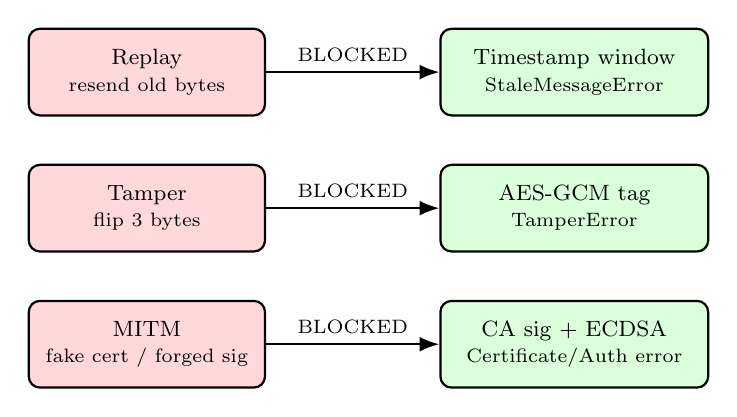
\begin{tikzpicture}[font=\footnotesize,node distance=5mm,
   atk/.style={draw,thick,rounded corners,fill=red!15,minimum width=3.0cm,
               minimum height=1.1cm,align=center},
   def/.style={draw,thick,rounded corners,fill=green!14,minimum width=3.4cm,
               minimum height=1.1cm,align=center}]
  \node[atk] (r) {Replay\\\scriptsize resend old bytes};
  \node[atk,below=6mm of r] (t) {Tamper\\\scriptsize flip 3 bytes};
  \node[atk,below=6mm of t] (m) {MITM\\\scriptsize fake cert / forged sig};
  \node[def,right=22mm of r] (rd) {Timestamp window\\\scriptsize StaleMessageError};
  \node[def,right=22mm of t] (td) {AES-GCM tag\\\scriptsize TamperError};
  \node[def,right=22mm of m] (md) {CA sig + ECDSA\\\scriptsize Certificate/Auth error};
  \draw[-{Latex[length=2.5mm]},thick] (r) -- (rd) node[midway,above,font=\scriptsize]{BLOCKED};
  \draw[-{Latex[length=2.5mm]},thick] (t) -- (td) node[midway,above,font=\scriptsize]{BLOCKED};
  \draw[-{Latex[length=2.5mm]},thick] (m) -- (md) node[midway,above,font=\scriptsize]{BLOCKED};
\end{tikzpicture}
\end{center}

\subsection{Diagram 2 --- the replay attack timeline}
\begin{center}
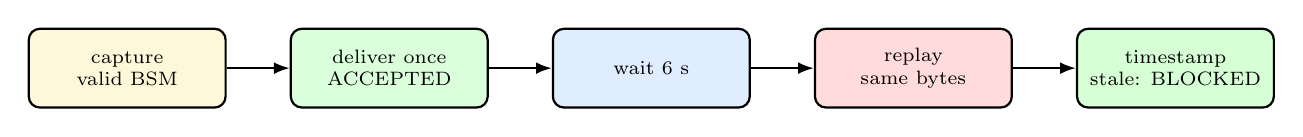
\begin{tikzpicture}[font=\scriptsize,node distance=4mm,
   s/.style={draw,thick,rounded corners,minimum width=2.5cm,minimum height=1.0cm,
             align=center}]
  \node[s,fill=boxyellow] (cap) {capture\\valid BSM};
  \node[s,fill=green!14,right=8mm of cap] (ok) {deliver once\\ACCEPTED};
  \node[s,fill=boxblue,right=8mm of ok] (wait) {wait 6 s};
  \node[s,fill=red!14,right=8mm of wait] (rep) {replay\\same bytes};
  \node[s,fill=green!16,right=8mm of rep] (blk) {timestamp\\stale: BLOCKED};
  \draw[-{Latex[length=2mm]},thick] (cap)--(ok);
  \draw[-{Latex[length=2mm]},thick] (ok)--(wait);
  \draw[-{Latex[length=2mm]},thick] (wait)--(rep);
  \draw[-{Latex[length=2mm]},thick] (rep)--(blk);
\end{tikzpicture}
\end{center}

% =====================================================================
\section{Presentation Pack}
% =====================================================================

\subsection{Slide Outline}

\textbf{Slide 1 --- Why Attack Your Own System?}
\begin{itemize}
  \item A security claim is worthless until tested.
  \item S8 is the project's red team --- three attack scripts.
  \item Each becomes the attacker against the real code.
  \item \texttt{[BLOCKED]} = the defence held; \texttt{[FAIL]} = it broke.
\end{itemize}

\textbf{Slide 2 --- The Replay Attack.}
\begin{itemize}
  \item Capture a valid message, wait 6 seconds, re-send it.
  \item The message is perfectly valid --- just \emph{old}.
  \item Timestamp check: 6\,s $>$ 5\,s $\to$ \texttt{StaleMessageError}.
  \item Result: replay BLOCKED.
\end{itemize}

\textbf{Slide 3 --- The Tamper Attack.}
\begin{itemize}
  \item Encrypt a BSM, flip 3 random bytes in the ciphertext.
  \item AES-GCM tag no longer matches $\to$ \texttt{TamperError}.
  \item The original, untouched message still decrypts fine.
  \item Result: tamper BLOCKED.
\end{itemize}

\textbf{Slide 4 --- The Man-in-the-Middle Attack.}
\begin{itemize}
  \item Scenario A: fake self-signed certificate $\to$ \texttt{CertificateError}.
  \item Scenario B: forged challenge signature $\to$ \texttt{ecdsa\_verify} False.
  \item Attacker lacks the CA key and the vehicle's private key.
  \item Result: both scenarios BLOCKED.
\end{itemize}

\textbf{Slide 5 --- Why the Attacker Always Loses.}
\begin{itemize}
  \item Every attack fails for one reason: a missing secret.
  \item No session key, no CA key, no vehicle private key.
  \item Honest limits: in-process tests, not a live network attack.
  \item The demos prove the crypto, not an exhaustive security proof.
\end{itemize}

\subsection{Speaker Talking Points (about 30--60 seconds each)}

\textbf{Slide 1.} ``It is easy to \emph{say} a system is secure. It means nothing
until someone genuinely tries to break it. Section eight is exactly that --- the
project's red team. There are three scripts, and each one becomes the attacker.
They do not use a watered-down copy of the code; they import the real project
modules and attack them. If a defence failed, the script would print FAIL in
capital letters. Every time, it prints BLOCKED.''

\textbf{Slide 2.} ``First, the replay attack. The attacker records a genuine,
valid, encrypted message. Notice --- nothing is forged here; the message is
completely legitimate. The script delivers it once, and it is accepted, proving
it is valid. Then it waits six seconds and sends the exact same bytes again. Now
the message's timestamp is six seconds old, and our freshness window is five.
secure\_receive raises a StaleMessageError. The replay is blocked --- not because
the message is fake, but because it is old.''

\textbf{Slide 3.} ``Second, the tamper attack. The script encrypts a safety
message, then plays the attacker: it flips three random bytes in the middle of
the packet, in the ciphertext region. Then it tries to receive it. AES-GCM
recomputes its authentication tag, the tag does not match the changed bytes, and
secure\_receive throws a TamperError. To prove the rejection is really caused by
the tampering, the script then decrypts the \emph{original} untouched message ---
and that one works perfectly. Only the tampered copy fails.''

\textbf{Slide 4.} ``Third, the man-in-the-middle, in two flavours. In Scenario A
the attacker builds their own certificate claiming to be vehicle-a. But they
cannot sign it as the CA --- they do not have the CA's key --- so it is
self-signed, and our certificate check raises a CertificateError. In Scenario B
the attacker lets the real certificates through but tries to answer the handshake
challenge by signing the nonces with their own key. When we verify that signature
with vehicle-a's real public key, it returns False. Both scenarios blocked.''

\textbf{Slide 5.} ``Step back and notice the pattern. Every single attack fails
for the same root reason: the attacker is missing a secret. They do not have the
session key, so they cannot tamper. They do not have the CA's key, so they cannot
forge a certificate. They do not have the vehicle's private key, so they cannot
forge a signature. And to be honest about the limits: these scripts run in one
process against the library functions, so they prove the cryptography is sound,
not that the networking is flawless, and they test the specific attacks we chose
rather than every possible attack.''

\subsection{Live-Demo Script}
\begin{enumerate}
  \item \textbf{Replay.} Run \texttt{python attacks\textbackslash
        replay\_attack.py}. Point at \texttt{First delivery ACCEPTED} (valid),
        the 6-second countdown, then \texttt{[BLOCKED] ... Message is 6.0s old}.
  \item \textbf{Tamper.} Run \texttt{python attacks\textbackslash
        tamper\_attack.py}. Point at the three flipped byte positions, then
        \texttt{[BLOCKED] ... auth tag mismatch}, then the original still decrypts.
  \item \textbf{MITM.} Run \texttt{python attacks\textbackslash mitm\_attack.py}
        (certificates must exist). Point at the two \texttt{[BLOCKED]} lines ---
        one for the fake certificate, one for the forged signature.
  \item \textbf{Optional break-it.} Change the replay wait to 3 seconds and show
        the message is now accepted --- explaining the timestamp window.
\end{enumerate}

\subsection{Examiner Q\&A}
\begin{enumerate}
  \item \textbf{Q: Why does the project include attack scripts at all?}\\
        A: To \emph{prove} the defences by adversarial testing. A claimed defence
        is only credible once a real attack against the real code is shown to
        fail.
  \item \textbf{Q: In the replay attack, is the message forged?}\\
        A: No --- it is a genuine, validly encrypted and signed message. The only
        thing wrong is that it is old; the timestamp window catches it.
  \item \textbf{Q: How exactly does the tamper attack get blocked?}\\
        A: Flipping bytes changes the ciphertext; AES-GCM's recomputed
        authentication tag no longer matches, \texttt{aes\_gcm\_decrypt} raises
        \texttt{DecryptionError}, and \texttt{secure\_receive} raises
        \texttt{TamperError}.
  \item \textbf{Q: Why does the tamper script also decrypt the original?}\\
        A: As a control --- it proves the channel works and that the rejection
        was caused specifically by the tampering, not a setup error.
  \item \textbf{Q: What are the two MITM scenarios and what blocks each?}\\
        A: (A) A fake self-signed certificate, blocked by
        \texttt{verify\_certificate\_against\_ca} (no CA signature). (B) A forged
        challenge signature, blocked by \texttt{ecdsa\_verify} with the real
        public key.
  \item \textbf{Q: What single thing does the attacker always lack?}\\
        A: A required secret --- the session key, the CA's private key, or the
        vehicle's private key. Without it, no attack succeeds.
  \item \textbf{Q: A replay within 5 seconds --- would this script catch it?}\\
        A: Not by itself: the timestamp would pass and \texttt{secure\_receive}
        does not consult the nonce cache. Catching that needs the nonce-cache
        layer, which the handshake (S4) uses.
  \item \textbf{Q: Name a limitation of these demonstrations.}\\
        A: They run in one process against library functions, not a live TCP
        connection, and they test chosen attacks --- so they evidence the
        cryptographic defences rather than constitute an exhaustive proof.
\end{enumerate}

% =====================================================================
\section{Glossary}
% =====================================================================
\begin{description}[style=nextline,leftmargin=0pt]
  \item[Adversarial testing] Deliberately attacking your own system to test it.
  \item[Red team] The people (or scripts) that play the attacker.
  \item[Replay attack] Re-sending a previously captured valid message.
  \item[Tamper attack] Changing a message's bytes in transit.
  \item[MITM] Man-in-the-Middle: an attacker secretly between two parties.
  \item[Self-signed certificate] A certificate signed with its own key, not the CA's.
  \item[Forged signature] A signature made with the wrong (attacker's) private key.
  \item[Freshness window] The 5-second age limit on a valid message.
  \item[Authentication tag] The 16-byte AES-GCM value that detects tampering.
  \item[Sequence number] A per-sender counter that must always increase.
  \item[StaleMessageError] Exception for a message older than the window.
  \item[TamperError] Exception for a packet that failed an integrity check.
  \item[CertificateError] Exception when certificate verification fails.
  \item[XOR / \^{}=] The bitwise operation used to flip bits when tampering.
  \item[bytearray] A mutable sequence of bytes (so it can be edited).
  \item[Session key] The shared 32-byte AES key (here simulated for the demos).
  \item[CA] Certificate Authority --- whose private key the attacker lacks.
  \item[Chain of trust] The signature link from a certificate to the trusted CA.
  \item[ecdsa\_verify] The function that returns False for a forged signature.
  \item[verify\_certificate\_against\_ca] The function that rejects a non-CA-signed cert.
\end{description}

% =====================================================================
\section{References and Further Study}
% =====================================================================
\begin{itemize}
  \item \textbf{Replay attack (Wikipedia)} ---
        \url{https://en.wikipedia.org/wiki/Replay_attack}\\
        Read for: how replay works and standard defences.
  \item \textbf{Man-in-the-middle attack (Wikipedia)} ---
        \url{https://en.wikipedia.org/wiki/Man-in-the-middle_attack}\\
        Read for: the MITM concept behind both scenarios.
  \item \textbf{Tampering / message integrity (Wikipedia: Data integrity)} ---
        \url{https://en.wikipedia.org/wiki/Data_integrity}\\
        Read for: why detecting modification matters.
  \item \textbf{Red team (Wikipedia)} ---
        \url{https://en.wikipedia.org/wiki/Red_team}\\
        Read for: the idea of adversarial testing.
  \item \textbf{Penetration test (Wikipedia)} ---
        \url{https://en.wikipedia.org/wiki/Penetration_test}\\
        Read for: professional security testing of which these scripts are a tiny version.
  \item \textbf{OWASP Web Security Testing Guide} ---
        \url{https://owasp.org/www-project-web-security-testing-guide/}\\
        Read for: how real-world security testing is structured.
  \item \textbf{Galois/Counter Mode (Wikipedia)} ---
        \url{https://en.wikipedia.org/wiki/Galois/Counter_Mode}\\
        Read for: why a flipped byte breaks the AES-GCM tag.
  \item \textbf{X.509 (Wikipedia)} ---
        \url{https://en.wikipedia.org/wiki/X.509}\\
        Read for: why a self-signed certificate fails the CA check.
  \item \textbf{Python cryptography --- exceptions} ---
        \url{https://cryptography.io/en/latest/exceptions/}\\
        Read for: \texttt{InvalidSignature} and \texttt{InvalidTag}, the errors
        behind the rejections.
  \item \textbf{MITRE ATT\&CK --- Adversary-in-the-Middle} ---
        \url{https://attack.mitre.org/techniques/T1557/}\\
        Read for: how MITM is catalogued as a real-world technique.
\end{itemize}

\vfill
\begin{center}\footnotesize\itshape
End of Section S8. Next: S9 --- the security evaluation that measures how well
these defences perform.
\end{center}

\end{document}
